% !TeX root = ../main.tex

\section{Numerical Results}
    \frame{\sectionpage}
      
    \begin{frame}{Performances of Different Policies}
        \scriptsize
        \begin{table}[ht]
          \centering
          \begin{tabular}{|l|l|l|l|l|l|l|}
          \hline
           T & Probabilities & SPP(\%) & DP1(\%) & Bid(\%) & Booking(\%) & FCFS(\%) \\
          \hline
          60  & [0.25, 0.25, 0.25, 0.25]  & 99.12 & 98.42 & 98.38 & 96.74 & 98.17 \\
          70  & [0.25, 0.25, 0.25, 0.25]  & 98.34 & 96.87 & 96.24 & 97.18 & 94.75 \\
          80  & [0.25, 0.25, 0.25, 0.25]  & 98.61 & 95.69 & 96.02 & 98.00 & 93.18 \\
          90  & [0.25, 0.25, 0.25, 0.25]  & 99.10 & 96.05 & 96.41 & 98.31 & 92.48 \\
          100 & [0.25, 0.25, 0.25, 0.25]  & 99.58 & 95.09 & 96.88 & 98.70 & 92.54 \\
          \hline
          60  & [0.25, 0.35, 0.05, 0.35]  & 98.94 & 98.26 & 98.25 & 96.74 & 98.62 \\
          70  & [0.25, 0.35, 0.05, 0.35]  & 98.05 & 96.62 & 96.06 & 96.90 & 93.96 \\
          80  & [0.25, 0.35, 0.05, 0.35]  & 98.37 & 96.01 & 95.89 & 97.75 & 92.88 \\
          90  & [0.25, 0.35, 0.05, 0.35]  & 99.01 & 96.77 & 96.62 & 98.42 & 92.46 \\
          100 & [0.25, 0.35, 0.05, 0.35]  & 99.23 & 97.04 & 97.14 & 98.67 & 92.00 \\
          \hline
          60  & [0.15, 0.25, 0.55, 0.05]  & 99.14 & 98.72 & 98.74 & 96.61 & 98.07 \\
          70  & [0.15, 0.25, 0.55, 0.05]  & 99.30 & 96.38 & 96.90 & 97.88 & 96.25 \\
          80  & [0.15, 0.25, 0.55, 0.05]  & 99.59 & 97.75 & 97.87 & 98.55 & 95.81 \\
          90  & [0.15, 0.25, 0.55, 0.05]  & 99.53 & 98.45 & 98.69 & 98.81 & 95.50 \\
          100 & [0.15, 0.25, 0.55, 0.05]  & 99.47 & 98.62 & 98.94 & 98.90 & 95.25 \\
          \hline
          \end{tabular}
        \end{table}
        SPP has better performance than other policies under different demands.

    \end{frame}
      
    \begin{frame}{Impact of Social Distancing as Demand Increases}
        \scriptsize
        $\gamma = p_1 * 1 + p_2 * 2 + p_3 * 3 + p_4 * 4$: the expected number of people at each period.
        \begin{figure}[h]
            \centering
            \subfigure[When $\gamma =2.5$]{
              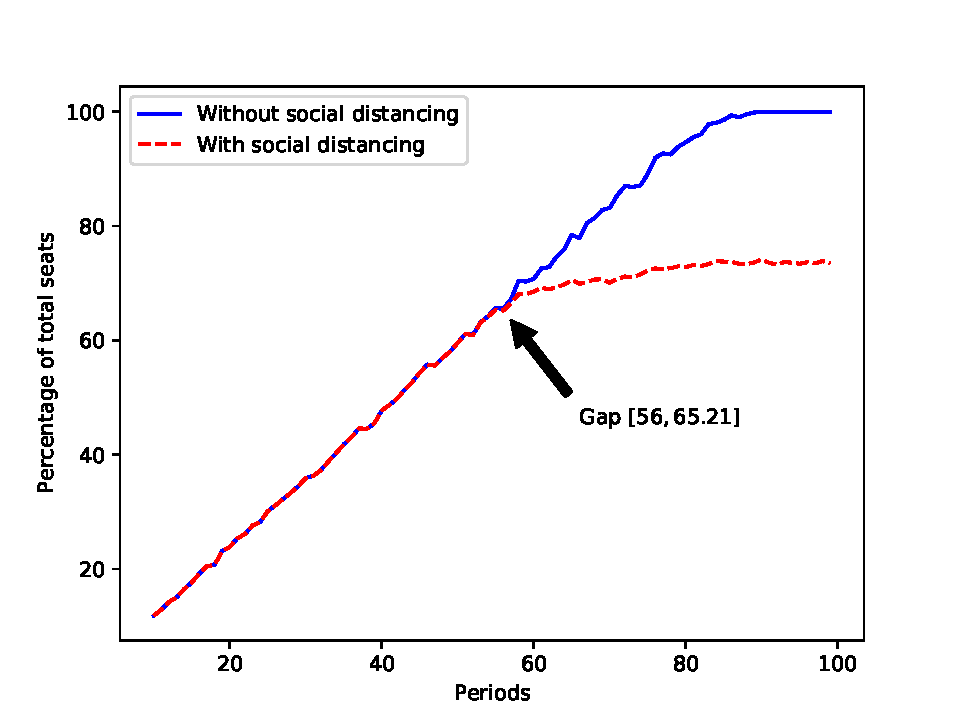
\includegraphics[width=0.48\textwidth]{./images/p1.pdf}}
            \subfigure[When $\gamma =1.9$]{
              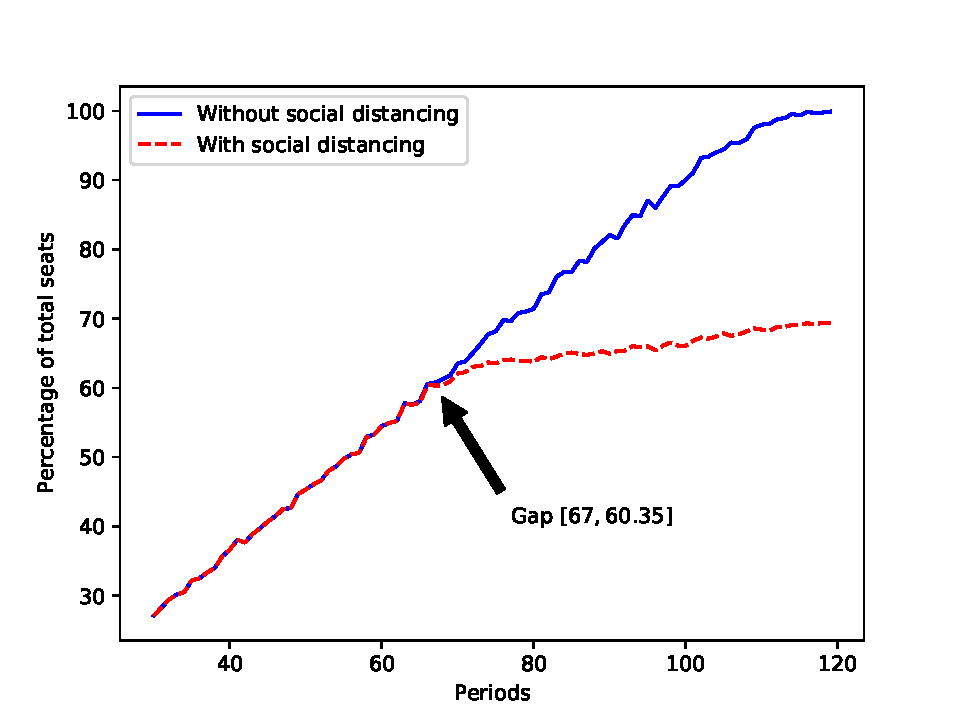
\includegraphics[width=0.48\textwidth]{./images/p2.pdf}}
          \end{figure}
        \scriptsize
        The gap point represents the first period where the number of people without social distancing is larger than that with social distancing and the gap percentage is the corresponding percentage of total seats.
    \end{frame}
      
    \begin{frame}{Estimation of Gap Point}
      \begin{figure}[ht]
        \centering
        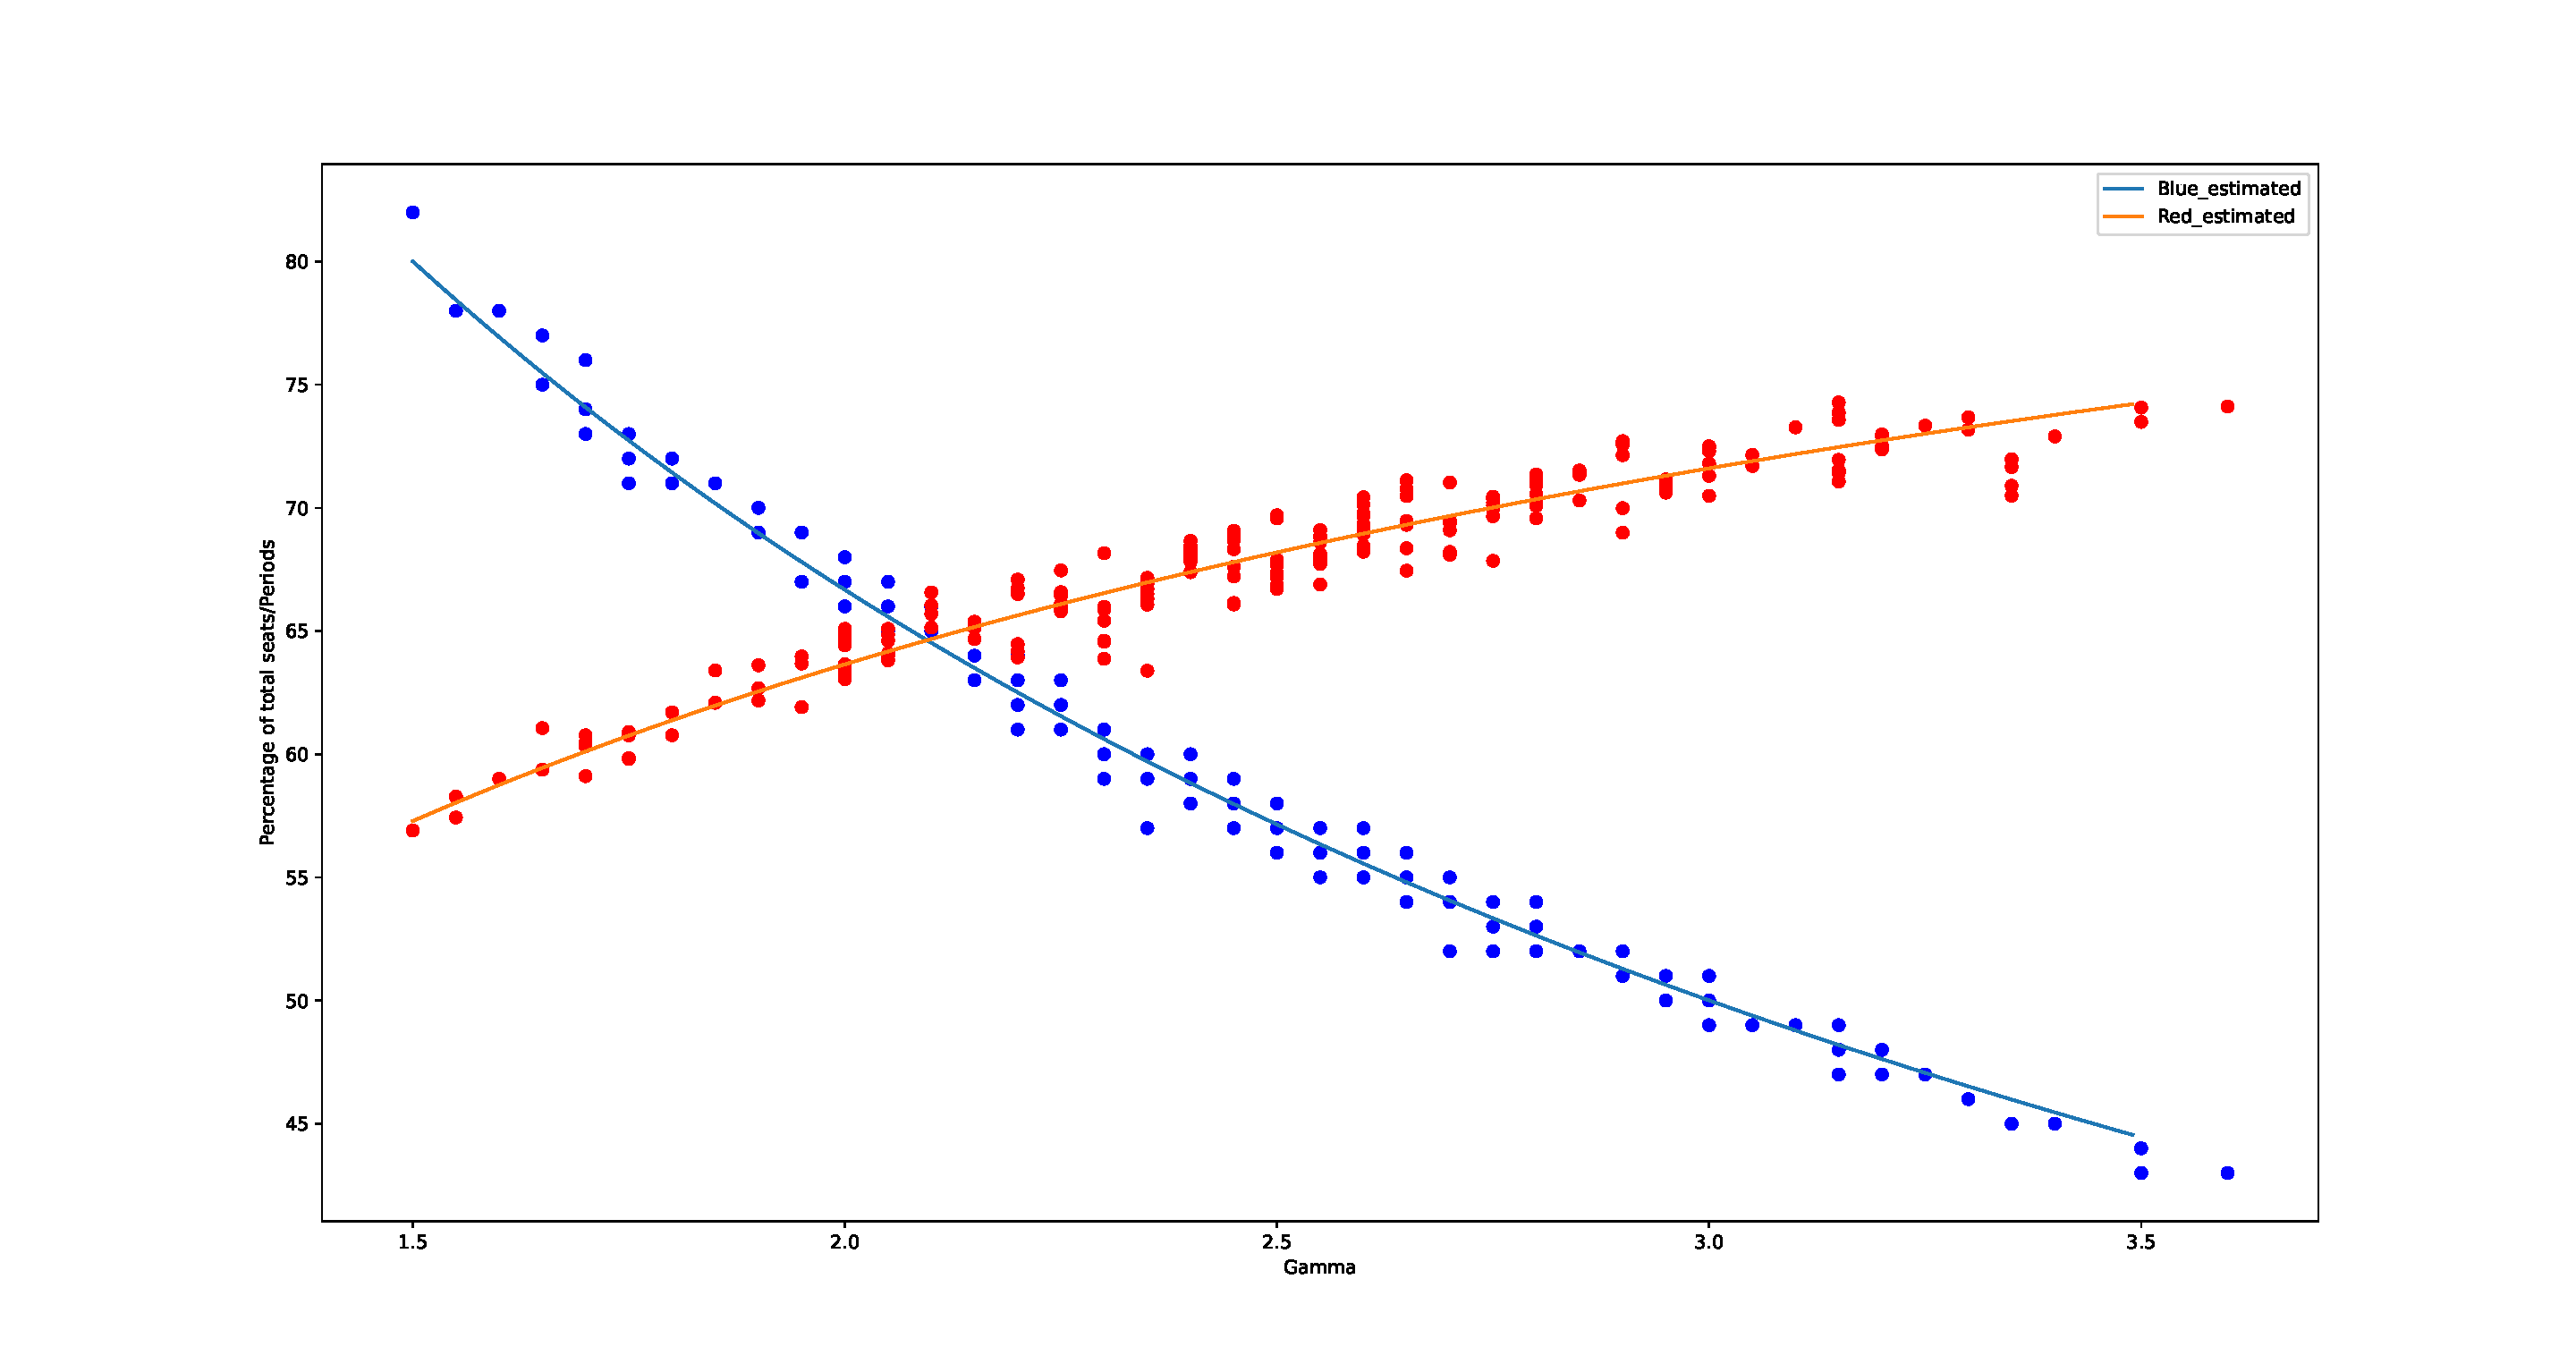
\includegraphics[width = 0.8\textwidth]{./images/gamma_estimation.pdf}
        \caption{Gap points under 200 probabilities}
    \end{figure}
    \scriptsize
    {\color{blue} Blue points}: period of the gap point.
    {\color{red} Red points}: occupancy rate of the gap point. 
    Gap points can be estimated.
    \end{frame}